\documentclass[output=paper]{langsci/langscibook} 
\author{Leah Geoghegan\affiliation{Portsmouth University}}
\title{International posture, motivation and identity in study abroad}
 
 
\abstract{In the context of Study Abroad (SA) researchers have called for a more refined analysis of students’ personal language learning motivations \citep{MitchellEtAl2015}. Furthermore, the spread of English as a Lingua Franca (ELF) has led to an exponential increase in learners of English, and has consequently changed the learners’ motivations for learning, as well as the way they identify with the language (\citealt{JenkinsEtAl2011,Isabelli-García2006}). With this in mind, the present study draws on \citegen{Yashima2009} international posture as a more fruitful alternative to the concept of integrative motivation. The study investigates the motivation and identity of undergraduate Spanish-Catalan bilinguals, learning English, as well as either German or French. Using quantitative tools, the study compares students cross-sectionally prior to and at the end of a SA period, and contrasts those spending a SA in an English-speaking country with those in a German- or French-speaking country. The results suggest that there is a partial effect of a three-month SA on the language learning motivation and identity of higher education students. Significant differences were found between pre- and end of SA participants in areas such as international posture, willingness to communicate and interest in foreign languages. Furthermore, when comparing those in an English-speaking country with a French or German-speaking country, differences arose regarding the ideal L2 self and intended learning effort. It is suggested that due to the generally high levels of motivation across all participants, a more detailed, qualitative investigation is required in order to gain a more thorough understanding of the development and negotiation of the learners' ongoing motivational process \citep{Kim2009}.}
\maketitle

\begin{document}
  

% \textit{Keywords}: Identity, Motivation, International Posture, Study \isi{Abroad}


\section{Introduction}

Within the field of Second Language Acquisition (\isi{SLA}) and \isi{Study Abroad} (SA), there has been a recent increase in interest regarding research examining individual factors such as identity (e.g. \citeauthor{Jackson2008b} \citeyear*{Jackson2008b}; \citealt{Kinginger2013,Brown2013}) and motivation (e.g. \citealt{Isabelli-García2006,Allen2010,Hernández2010,Sasaki2011,IrieRyan2014}), an unsurprising fact given that “ethnographic and {post-structuralist} thinking have become increasingly influential within \isi{SLA} theorising” in recent decades \citep[8]{MitchellEtAl2015}. The international role of \ili{English} as a Lingua Franca (\isi{ELF}) in SA and higher education contexts has also seen increasing attention in research over the last decade (e.g. \citealt{Smit2010,Jenkins2011,Coleman2015}), in part due to the increase in \ili{English} medium instruction in tertiary education outside \ili{English}-speaking countries. 

What has been called for in this field of research, is a more refined investigation into students’ personal language learning motivations \citep{MitchellEtAl2015}. This analysis is particularly necessary as a result of the spread of \isi{ELF}, which has changed the learners’ motivations for learning as well as the way they identify with the language (\citealt{JenkinsEtAl2011}; \citealt{Isabelli-García2006}). As \citet[2]{Melitz2016} points out, “there has never been in the past a language spoken more widely in the world than \ili{English} is today.” What is more, in 2013 the number of people actively learning \ili{English} at a useful level was estimated at 1.75 billion people worldwide, and this figure is predicted to reach 2 billion by 2020 (\citealt{BritishCouncil2013}). However, the importance of the language does not only affect the number of people who learn it, but also the way in which it is taught and learned. The emergence of concepts such as World Englishes (WE) and \isi{ELF} have challenged the traditional \ili{English} language teacher paradigm \citep{Pakir2009}, wherein the ultimate objective was often the unrealistic ideal of native-like competence (\citealt{KeCahyani2014}). It has been suggested that concepts such as \isi{ELF} may lead to a reconsideration of these traditional \isi{native speaker} models \citep{Seidlhofer2001}, in that the language learner, rather than aspiring towards native-like \isi{proficiency}, could instead aim towards becoming a proficient, international \ili{English} speaker \citep{Majanen2008}. This approach seems appropriate, given that native-speaker norms and usages are often not relevant in the context of an international \isi{ELF} exchange (\citealt{KeCahyani2014}), as individuals may be more concerned with being understood rather than speaking like a \isi{native speaker}. 

This alternative approach will evidently affect the language learner, both in how they identify with their \isi{target language} (TL), as well as their motivation to learn. Regarding identity, it has been suggested that \isi{ELF} may offer a more attractive identity to the non-\isi{native speaker}, given that “instead of perpetual \textit{learners} of \ili{English}, they can now regard themselves as legitimate \ili{English} \textit{users} in the international world” \citep[2]{Majanen2008}. As for motivation, there are at least two repercussions as a result of \isi{ELF} (\citealt{DörnyeiUshioda2013}). Firstly, given that speaking \ili{English} is increasingly viewed as a basic educational skill crucial to economic and professional advancement, a learner’s motivation for learning \ili{English} is likely different from that of learning other languages. This issue is highlighted by \citet{BlockCameron2002} who discuss how language learning and communication skills that are demanded by globalisation influence the learners’ motivation towards instrumentality. Secondly, \citet[135]{GardnerLambert1972} highlight the importance of \isi{integrative motivation}, stating that a motivated learner “must be willing to identify with members of another ethnolinguistic group and take on very subtle aspects of their behaviour.” However, this \isi{concept of integrative motivation} makes little sense when discussing \isi{ELF} learners, who may instead focus on communication with speakers of different {linguistic} backgrounds \citep{Breiteneder2005}. In such a context, traditional concepts in motivation research such as integrativeness and attitudes toward the \isi TL community become increasingly obscure, given that it becomes more and more difficult for \isi{ELF} learners to identify with a clear target group or culture \citep{Yashima2009}. Consequently, when it comes to \isi{ELF}, it may make more sense to evaluate students’ motivation based on their international \isi{posture}, that is, the “tendency to see oneself as connected to the international community” \citep[3]{Yashima2009}, rather than a specific second language (\isi{L2}) group. For example, in the context of a European SA, native \ili{Spanish} speakers studying abroad in the UK can interact in \ili{English} with both native \ili{English} speakers, as well as other non-native speakers using \isi{ELF}. In such a context, these students may not (solely) be motivated to improve their language skills in order to become integrated in the \isi{native speaker} community. Their language motivation may also be driven by a desire to become integrated into a community of \isi{ELF} users in an Erasmus “community of practice” \citep{Wenger1998}. As \cite{KaypakOrtaçtepe2014} point out, due to the growing number of Erasmus students studying abroad in such \isi{ELF} communities, what is needed is a closer look into the use of \ili{English} in these communities.

With this in mind, this study takes a cross-sectional approach, using quantitative research tools to investigate the identity and motivation of the language learners in the context of SA, by exploring the differences between pre- and end-of SA students, and between language learning in an \ili{English}-speaking country compared to a French/\ili{German}-speaking country. The participants in the study are \ili{Spanish}-\ili{Catalan} bilinguals, learning \ili{English}, as well as either \ili{German} or French as part of their undergraduate degree, and who spent a semester abroad in an \ili{English}-, \ili{German}- or French-speaking country.


\section{Literature review}

The following three sections provide an overview of the relevant literature for this study: the fields of SA, identity and motivation.

\subsection{Study Abroad}


Since the second half of the twentieth century, there has been an exponential development of a global market in international education (\citealt{MazzarolEtAl2003}). This surge of internationalisation naturally has also included the encouragement and increase of SA programmes \citep{Jackson2008a}. For example, within the European context, one of the key features of the European {linguistic} policy towards \isi{multilingualism} “has been the promotion of student mobility across Europe” \citep[103]{Pérez-Vidal2011}.

As \citet{Jackson2008b} points out, much of SA research to date has been dominated by statistical studies that have focused on {linguistic} outcomes and \isi{grammatical} development, while, according to \citet{Coleman1998}, essential components of \isi{proficiency}, such as \isi{sociocultural} and \isi{intercultural} competence, have been largely neglected. \citet[165]{CollentineFreed2004intro} also point to this issue, highlighting the need to better define “the social conditions surrounding, affecting and perhaps impeding learner gains.”

This call has led SA research to change its trajectory from “identifying and quantifying {linguistic} gains (or lack of) to exploring the experience of SA from an ethnographic perspective” \citep[6]{Devlin2014studyabroad}. Recent research has thus seen an increase in introspective techniques such as diary studies, first-person narratives and interviews, as well as case studies and ethnographies, in an effort to better understand the processes involved in language learning \citep{Jackson2008b}. As \citet{Devlin2014studyabroad} points out, this “learner-centric” approach has allowed researchers such as \citet{Isabelli-García2006}, \citet{Jackson2008b} and \citet{Kinginger2004} to underscore the specific factors which aid or inhibit a learner’s language \isi{acquisition} and access to native speakers. More recently, \citet[134]{MitchellEtAl2015} have called for a “more refined analysis of students’ personal motivations and characteristics, \isi{multilingual} language practices, and emerging social relations” with the aim of explaining the variation in the \isi{L2} development of  SA participants. This \isi{learner-centric approach} reflects the “social turn” in \isi{SLA} \citep{Block2003}, and may aid in deciphering why there is “no evidence that one context of learning is uniformly superior to another for all students” (\citet[164]{CollentineFreed2004intro}). 



\subsection{Identity}


One facet of the above mentioned \isi{learner-centric approach} is the issue of identity. According to Oxford Dictionaries, the term identity can be used to describe “the fact of being who or what a person or thing is" (Identity [Def.1] 2016), and also "a close similarity or affinity” (Identity [Def.2] 2016). Many researchers now define identity as a process, due to the fact that individual identities are not fixed states, but rather “are negotiated, or performed, in the interplay of the relationships between individuals and their social contexts” \citep[11]{Stockton2015}. As regards \isi{SLA}, both an \isi{L2} learner’s individual identity and also how they identify with the culture of the TL are of particular interest. \isi{L2} motivation researchers “have always believed that a \isi{foreign language} is more than a mere communication code […] and have therefore typically adopted paradigms that linked the \isi{L2} to the individual’s personal ‘core’, forming an important part of one’s identity” \citep[9]{DörnyeiUshioda2009}.

Many researchers have highlighted the importance of the degree to which the learner identifies with the TL, finding that in many cases a positive identification with the TL and target culture results in successful language \isi{acquisition} (e.g. \citealt{Regan2013,Norton2000,NestorRegan2011,NestorEtAl2012}), while negative identification results in unsuccessful language \isi{acquisition} (e.g. \citealt{Norton2000,Block2006}). Informal language learning and its impact on the learner’s identity is thus of particular interest, given that “the sustained \isi{immersion} in a new cultural and {linguistic} milieu seemingly cannot but impact on the individual’s sense of self” \citep[109]{Block2007}.

The \isi{learning context} of SA is one such environment that may challenge the learner’s identity. Having been taken out of their ‘comfort zone’, and thrown into an entirely different {linguistic} milieu, learners often struggle with their sense of identity \citep{Jackson2008b}. According to \citet[202]{Kinginger2009}, the value of SA as a learning environment depends on “whether [the student’s] encounters lead to frustration or to the desperate, creative longing to craft a foreign language-mediated identity.” It is possible that the way in which students manage this impact on their sense of self will ultimately determine the success of their language \isi{acquisition}. Thus, by investigating these individual experiences, researchers may be able to interpret the varying results of SA students' lives.



\subsection{Motivation}


As with identity, research has also shown that motivation is a key factor in students’ learning \citep{Keblawi2009}. As pointed out by \citet{Dörnyei2014}, even language learners with the most remarkable abilities will be unable to accomplish long term goals if they lack the motivation to do so.  

According to \citet{UshiodaDörnyei2012}, there have been four different stages in the history of motivation research in foreign \isi{language teaching} and learning, as summarised in \tabref{tab:geoghegan:1}. 

\begin{table}
\begin{tabularx}{\textwidth}{QlQ}
\lsptoprule
\bfseries Stage & \bfseries Timeline & \bfseries Characteristics\\
\midrule 
(1)
         The social psychological period & 1959-1990 & Proposes two kinds of motivational orientation: integrative and instrumental.\\
\tablevspace         
(2)
         The cognitive-situated period & During the 1990s & Draws from cognitive theories in educational psychology \\
\tablevspace         
(3)
         The process-oriented period & Turn of the century & Focuses on motivational change\\
\tablevspace         
(4)
         The socio-dynamic period & Current & Concerned with dynamic systems and contextual interactions\\
\lspbottomrule
\end{tabularx}
%%[Warning: Draw object ignored]
%%[Warning: Draw object ignored]
\caption{Four stages in the history of motivation research, adapted from \citet{UshiodaDörnyei2012}.}
\label{tab:geoghegan:1}
\end{table}

The current stage, the socio-dynamic period, which has developed over the last decade, has given rise to three new conceptual approaches (\citealt{UshiodaDörnyei2012}), namely 
(i) Ushioda’s (\citeyear{Ushioda2009}) person-in-context relational view of \isi{L2} motivation, 
(ii) motivation from a complex dynamic systems perspective (\citealt{WaningeEtAl2014}), and 
(iii) Dörnyei’s (\citeyear{Dörnyei2009}) \isi{L2} \isi{motivational} self system, which will be central to the current study. This system is influenced by two key psychological concepts, namely \citeapo{MarkusNurius1986} theory of \textit{possible selves} and \citeapo{Higgins1987} theory of \textit{ought selves.} The \isi{L2} \isi{motivational} self system fuses aspects of these two concepts and draws on the idea that an individual’s motivation is made up of the following three key parts:

\begin{enumerate}
\item The \textit{\isi{Ideal L2 Self}:} the image one has of their future self as an \isi{L2} user according to their own wishes. This component typically fosters integrative and internalised motives (e.g. ‘I am motivated to learn \ili{Spanish} because I see myself being surrounded by lots of \ili{Spanish} friends.’). 
\item The \textit{Ought-to \isi{L2} Self:} the image one has of their future self as an \isi{L2} user according to external expectations. This facet deals with attributes which the learner believes they \textit{ought to} possess in order to meet expectations and avoid negative outcomes. This component reflects more extrinsic types of \isi{instrumental motivation} (e.g. ‘I need to work hard at learning my \isi{L2} so that I don’t disappoint my parents.’).
\item The \textit{\isi{L2} learning experience:} concerned with volition, or ‘executive’ motives, that is, “motivational influences that operate during task engagement, facilitating or impeding goal-directed behavior.” (\citealt{DörnyeiOttó1998}: 45). Such influences may include the impact of the language teacher, curriculum, peer group, experience of success or failure, etc. (e.g. ‘I don’t want to learn French because my teacher is not very nice and I always get bad grades.’).

\end{enumerate}


\largerpage
Within this motivational self system, both \isi{instrumental motivation} (i.e. wanting to learn a language for some practical purpose such as economic or educational advancement) and \isi{integrative motivation} (i.e. the desire to learn a language in order to communicate with the language's speakers and out of an interest in the language's culture) play a key role. However, regarding \isi{ELF}, the role of \isi{integrative motivation} may undergo a drastic change given that learners of \ili{English} are perhaps less inclined to see themselves integrating with native speakers than with other non-native \ili{English} speakers, as discussed above. This issue has been highlighted by \citet[7]{Dailey2009}, who states that “due to the change in global languages, there is no model community to identify with, consequently leading to a broader classification of \isi{integrative motivation}.” This implies that in a context of international students using \ili{English} as a common language, it makes little sense to gauge the extent to which these students wish to integrate with a native \ili{English}-speaking community. To resolve this issue, international \isi{posture} has been offered as an alternative to \isi{integrative motivation} \citep{Yashima2009}, a concept which captures the learners’ tendency to relate themselves to an international community rather than a specific \isi{L2} group. In other words, it captures “a tendency to see oneself as connected to the international community, have concerns for international affairs and possess a readiness to interact with people [of different nationalities]” \citep[3]{Yashima2002}. Yashima introduced this term in relation to \ili{Japanese} students learning \ili{English} in Japan. The context at hand, however, differs in that students studying abroad may have both the option of integrating with native \ili{English} speakers, and/or with other non-native \ili{English} users, with one situation at times appearing more attractive, for varying reasons. 

A final concept that is important here is that of Willingness to \isi{Communicate} (WTC), that is, the willingness of students to actively seek out opportunities to communicate in their \isi{TL}. WTC has been linked to both motivation and international \isi{posture}. For example, a study by \citet{Yashima2002} found that motivation affected self-confidence in \isi{L2} communication, which in turn led to increased WTC in the \isi{L2}. In addition, a significant link was found between International Posture (IP) and {WTC} in a \isi{L2}.

With the increasing dominance of socio-dynamic approaches in \isi{L2} motivation research, it is becoming increasingly evident that the dynamic individuality of the learners needs to be taken into account, as well as the fact that the students' identities, and their motivation, are in  constant change \citep{Guerrero2015}. Given that research to date has proven the \isi{Ideal L2 Self} and the \isi{L2} learning experience to be important components of the \isi{L2} \isi{motivational} self system (e.g. \citealt{TaguchiEtAl2009,IslamEtAl2013,KimKim2014}), while the ought-to self has been shown to be the least contributing factor (\citealt{IslamEtAl2013,Papi2010} as quoted in  \citealt{TortCalvo2015}), the current work will focus only on the two former components of the \isi{L2} \isi{motivational} self system. {IP} will also be investigated, in order to determine its effect on the participants' motivation. To this effect, the fourteen categories chosen for this study will reflect these issues, focusing on the \isi{Ideal L2 Self}, \isi{L2} Learning Experience, {WTC} and {IP}.


\section{The study}\label{sec:geoghegan:3}
\largerpage
The current study was carried out for two main reasons. Firstly, in order to begin to answer \citegen{MitchellEtAl2015} call for more a refined analysis of students’ personal motivations during SA. Secondly, to investigate what \citet{Kinginger2009} highlights as one of the most pressing issues for SA researchers: the effect of intensified globalization on language learning. In order to do so, the study has two objectives. Firstly, it compares two groups of students cross-sectionally, prior to and at the end of a \isi{SA} period. Secondly, focusing only on the second group of students who have completed their SA, this study contrasts those spending a SA in an \ili{English}-speaking country with those in a \ili{German}- or French-speaking country. The study puts forth the following research questions and hypotheses:

\begin{description}
 \item[RQ1.] Is there an effect of a three-month SA on the motivation and identity of higher education students who are sojourning in \ili{English}-, French- and \ili{German}-speaking countries? 
 \item[H1.] It is expected that there will be a difference between the identity and motivation of these students and those who have not spent a three-month period of studying abroad.

 \item[RQ2.] Is there an effect of a three-month SA on the motivation and identity of higher education students who are sojourning in an \ili{English}-speaking country as compared with a French- or \ili{German}-speaking country? 

 \item[H2.] It is expected that there will be a difference between the motivation and identity of students sojourning in \ili{English}-speaking countries compared to French- or \ili{German}-speaking countries, given that students studying \ili{English} may be more instrumentally motivated. 

\end{description}




\section{Methodology}

\subsection{Research approach and design}


The original design of the study aimed to capture the identity and motivation of SA students by means of quantitative data collections.

\begin{table}
\begin{tabular}{lll}
\lsptoprule

\multicolumn{3}{c}{ \bfseries Academic Year 2015-2016}\\
\midrule
\multicolumn{3}{c}{ \bfseries Year 1 of degree}\\
\midrule 
\fbox{\parbox{3cm}{Term 1\\Formal instruction}} & 
\fbox{\parbox{3cm}{Term 2\\Formal instruction}} &
\fbox{\parbox{3cm}{Term 3\\Formal instruction}} \\
\multicolumn{3}{c}{↑}\\
\multicolumn{3}{c}{Data collection 1: pre-SA}\\
\midrule 
\multicolumn{3}{c}{ \bfseries Year 2 of degree}\\
\midrule 
\fbox{\parbox{3cm}{Term 1\\Study abroad}} & 
\fbox{\parbox{3cm}{Term 2\\Formal instruction}} &
\fbox{\parbox{3cm}{Term 3\\Formal instruction}} \\
\multicolumn{1}{r}{↑}\\
\multicolumn{3}{c}{Data collection 2: End of SA}\\
\lspbottomrule
\end{tabular}
\caption{{Design}  {of}  {the}  {study}.}
\label{fig:geoghegan:graph1}
\end{table} 

\newpage 
The design of this study, outlined in \tabref{fig:geoghegan:graph1}, spanned across one academic year and was conducted with two groups of students in the first and second year of the same undergraduate degrees in order to collect data on motivation and identity from students before and after SA\footnote{Due to the time restrictions, it was not possible for a two-year longitudinal sample to be collected, and thus a cross-sectional design had to be adopted for the purposes of this study.}. More specifically, data collection took place in term 2, year 1 (Group 1, pre-SA), and in term 1, year 2 (Group 2, end of SA).

\subsection{Participants}


The participants in this study were \ili{Spanish}-\ili{Catalan} bilinguals (N=68) studying in the first or second year of their undergraduate degree. All participants were learning \ili{English} as a major language, as well as either French or \ili{German} as a minor language in their undergraduate degree. As part of their curriculum, the students completed one year of \isi{formal instruction}, followed by a compulsory three-month SA in a \isi{TL} country. The sojourn was organised by the university at the beginning of the second year of their degree and counted towards ECTS credits in their home university. The majority of the students were between 18 and 22 years old (\textit{M=}19.7) and were primarily female (10 male, 58 female), reflecting a demographic trend in language degrees.  

Group 1 (N=25) was made up of first year, pre-SA students. Group 2 (N=43) was made up of second year students of the same degree who were at the end of their SA at the time of the data collection. Both Group 1 and Group 2 completed the questionnaire concerning language background, motivation and identity. 

 
\subsection{Data collection}
\subsubsection{ Instruments: The questionnaire}

A questionnaire was used as the main instrument for data collection in this study (see Appendix 1). It was made up of a total of 116 questions: seven open questions concerning background information and the rest regarding issues concerning identity, motivation and WTC, with a five-level Likert scale format, offering five choices for each item ranging from ‘strongly agree’ to ‘strongly disagree’, or ‘absolutely true’ to ‘not true at all’ (\tabref{tab:geoghegan:2}). The questionnaire was written in \ili{English} given that the faculty of the participants’ degree programmes set a minimum standard of a B2.2 level in \ili{English} for admission, because students are expected to achieve a C1.1 by the end of their first year of formal instruction and a C1.2 by the end of their second year \citep{Beattie2014}. This level of \ili{English} was a requirement for all students including those who would \isi{SA} in a non-\ili{English}-speaking country. The Likert scale format was chosen, rather than a simple yes/no answer format, to allow room for manoeuvre, while at the same time maintaining control over the possible responses \citep{Bloomer2010}. 

\begin{table}
\small
\begin{tabularx}{\textwidth}{Q>{\centering}Q>{\centering}p{10mm}>{\centering}Q>{\centering}Qp{12mm}}
\lsptoprule
& absolutely true & mostly true & partly true partly untrue & not really true & not true at all \\
\midrule
33. In the future, I would like to participate in a volunteer activity to help foreigners living in the surrounding community. (155) & 
  $\square$
 & 
 $\square$
 & 
 $\square$
 & 
 $\square$
 &  
 ~~~~$\square$
\\
%%
\lspbottomrule
\end{tabularx} 
\caption{Sample questionnaire item using a five-level Likert scale format.}
\label{tab:geoghegan:2}
\end{table}

The questionnaire was based on \citegen{Ryan2009} and \citegen{Yashima2009} questionnaires, which were used to investigate the \isi{Ideal L2 Self} of \ili{English} learners in tertiary educational institutions. These questionnaires were chosen for two main reasons. Firstly, they investigated the \isi{Ideal L2 Self} while also incorporating elements that were relevant to the current study, including International Posture and Willingness to \isi{Communicate}. Secondly, variables had been piloted and were shown to have high internal reliability. 

The questionnaire, which consisted of a total of 14 categories, was divided into three sections: the first section dealt with personal details and general information. The second dealt with the categories \isi{WTC} in the native language (NL) and \isi{TL}, which was given its own section due to the large number of questions it contained, and the third with the remaining twelve. As discussed by  \citet[76]{DörnyeiCsizér2012}, the notion of multi-item scales, that is, the use of more than one item to address each identified content area, “is the central component in scientific questionnaire design.” With this in mind, the categories in the questionnaire were made up of multi-item scales of between three to eighteen items. Furthermore, items and scales were mixed throughout the questionnaire to create variety and prevent participants from simply repeating previous answers (\citealt{DörnyeiCsizér2012}).

Initial piloting of the item pool, which took the form of a think-aloud protocol, was carried out with three students in order to test the questionnaire. This process involved having the individuals answer the items in the questionnaire and provide feedback, after which the questionnaire was further revised prior to administration\footnote{Given the timeline of this study, the think-aloud protocol was considered the best piloting scenario available to the researcher, as a full piloting with the specific population it was intended for was not possible.}.

The original questionnaires by \citet{Ryan2009} and \citet{Yashima2009} were revised for the purposes of the current study in three main ways. Firstly, several categories were eliminated given that they were “only of peripheral interest but not directly related to the variables and hypotheses that the questionnaire has been designed to investigate” (\citealt{DörnyeiCsizér2012}: 76). Secondly, several questions were re-worded in order to create additional questions for \sectref{sec:geoghegan:3}, which contained two distinct parts: ‘While  {Abroad}’ (WA) and ‘In General’ (IG). In the section WA of the questionnaire, students were asked to specifically reflect on how they felt while abroad. These questions were used for comparison purposes with the original question found in \sectref{sec:geoghegan:3} IG, where the students were asked to reflect on their feelings in general. An example of this can be seen as follows:

\ea
{WA, Question 15: Using \ili{English}/French/\ili{German} in front of people on Erasmus makes me feel like I will be thought of as less \ili{Spanish}.} \\
{IG, Question 37: Using \ili{English}/French/\ili{German} in front of people in Spain makes me feel like I will be thought of as less \ili{Spanish}.}\\
\z

Thirdly, newly created questions were introduced in the section on ‘WA’, asking students to reflect on their {linguistic} improvement and ease of learning while abroad. The questionnaires for Group 1 and 2 were identical except for the fact that Group 2’s questionnaire included the additional ‘WA’ segment of \sectref{sec:geoghegan:3}, which dealt with reflection after time spent studying abroad. As Group 1 had not yet been abroad, this section was excluded from their questionnaire. Furthermore, Group 1 was instructed to indicate in which country they planned to do their SA, and to answer the questionnaire thinking specifically about the language spoken in that country, while Group 2 focused on the language of the country they were studying in at the time. Other than these two differences, the questionnaire and the order of the questions were the same for both groups.    

In order to determine the \isi{appropriateness} of the scales, reliability analyses were carried out following the study. Post hoc item analysis revealed that a number of items (six questions in total) did not work in the particular category, and were consequently removed in order to increase the scales´ internal reliability. Despite these exclusions, it was found that the Cronbach alpha values of some categories were not as high as they were in the source questionnaires, with five categories above .75, and nine ranging between .60 and .67 (see Appendix 2). As  \citet[95]{DörnyeiTaguchi2009} pointed out, “if the Cronbach alpha of a scale does not reach .60, this should sound warning bells”. Given that all categories were not below this figure, they were deemed acceptable for the purposes of the current study.


\subsubsection{Procedure}

The main criterion for taking the questionnaire was that the students must have been partaking in a SA, a compulsory component of the students’ undergraduate degrees. To this effect, convenience sampling was used in this study \citep{Dörnyei2007}, as the students who took the questionnaire all possessed the key characteristic relevant to the study: having spent an academic semester abroad \citep{Aiken1997}. Statistical consideration was also taken into account, with the sample including more than 30 people (\citealt{HatchLazaraton1991}). During the last month of their SA (Year 2, Term 1), the 44 participants that made up Group 2 answered the questionnaire via the online survey platform Qualtrics. The students were contacted via email to introduce the study and were sent a hyperlink to complete the online questionnaire, which took about fifteen to twenty minutes to complete. The students were also contacted at a later date in order to have them sign a consent form, indicating that they gave their approval for their data to be used in the study. The students were also informed that the results would be fully confidential, and that their personal data would not be used by or distributed to other parties.  The 25 Group 1 students were invited to take part in the questionnaire at the end of one of their university classes (Year 1, Term 2). All students signed the consent form at this time, and were then sent the hyperlink to complete the questionnaire.

 
\subsection{Data analysis}


The data gathered by means of the questionnaire were analysed using SPSS, version 23. When coding the questionnaire data, each response on the Likert scale was assigned a consecutive number, as suggested by \citet{DörnyeiCsizér2012}: numerical value 1 was assigned to 'strongly disagree', 2 to 'disagree', 3 to 'somewhat agree/somewhat disagree', 4 to 'agree', and 5 to 'strongly agree'. Before analysis, data cleaning and data manipulation were carried out. Negatively-worded items were re-coded by being reversed before analysis. For the first and second research questions, non-parametric, independent-samples Mann-Whitney U tests were carried out, given that the results of two independent groups (Group 1 pre-SA versus Group 2 end of SA, as well as students on SA in an \ili{English}-speaking country versus students on SA in a French- or \ili{German}-speaking country) were being compared, and the data were not normally distributed \citep{Dörnyei2007}. Non-parametric, paired samples Wilcoxon signed-rank tests were also carried out on the second year’s ‘While  {Abroad}’ and ‘In General’ comparison pairs, given that two sets of scores obtained from the same group were being compared, and the data were not normally distributed \citep{Dörnyei2007}. Alpha level was set to be at α =.05, as is typical in the \isi{SLA} literature (\citealt{Larson-Hall2012}).  


\section{Results}


\subsection{RQ1: SA vs. at home}


The first \isi{research question} in this study aimed to answer whether there was an effect of a three-month study abroad on the motivation and identity of higher education students sojourning in \ili{English}-, French- or \ili{German}-speaking countries. Results of Mann-Whitney U tests comparing the pre-SA Group 1 with the end of SA Group 2 showed a statistical difference in only 2 out of the 14 categories, along with 2 individual questions. These results are to be interpreted with caution, given the risk of obtaining significant results by chance when running multiple statistical tests. However, they point to some interesting trends in the data that merit discussion here and further investigation in future research. \tabref{tab:geoghegan:3} below shows the descriptive statistics with the means, the standard deviation and the statistics for the categories as well as the individual questions, which yielded significant results. In interpreting results, it should be borne in mind that higher numerical values correspond to ‘agree’ and ‘strongly agree’, while lower values correspond to low agreement. Three categories were relevant, namely (i) interest in foreign languages (IFL), (ii) international posture: having things to \isi{communicate} in the world (IPHTCW) and (iii) \isi{WTC} in the individual’s native language (WTCN). 

\begin{table}
\small
\begin{tabularx}{\textwidth}{Qrrrrrrrrrr}
\lsptoprule

\bfseries Question & \multicolumn{2}{c}{\bfseries M} & \multicolumn{2}{c}{\bfseries SD} & \bfseries \textit{U} & \bfseries \textit{z} & \bfseries \textit{p} & \multicolumn{2}{c}{\bfseries \textit{n\textsuperscript{2}}} & \bfseries \textit{d}\\
& \bfseries G1 & \bfseries G2 & \bfseries G1 & \bfseries G2 &  &  &  &  & \multicolumn{2}{c}{}\\
\midrule 
\textbf{WTCN\_Mean}: Mean of 9 statements on “Willingness to \isi{Communicate}’ in the students' L1 & 3.81 & 3.3 & .824 & 1.01 & 304.500 & 2.063 & .039 & 0.07 & \multicolumn{2}{c}{0.547}\\

\tablevspace
\textbf{IFL\_Mean:} Mean of 4 statements on ‘Interest in Foreign Languages’ & 5 & 4.3 & .000 & .1.28 & 387.500 & 2.874 & .004 & 0.054 & \multicolumn{2}{c}{0.476}\\

\tablevspace
\textbf{IFL\_31:} If I were visiting a foreign country I would like to be able to speak its language. & 5 & 4.7 & .000 & .513 & 387.500 & 2.885 & .004 & 0.054 & \multicolumn{2}{c}{0.476}\\

\tablevspace
\textbf{IPHTCW\_34}: I have thoughts that I want to share with people from other parts of the world. & 3.76 & 4.23 & .779 & .996 & 724.000 & 2.514 & .012 & 0.083 & \multicolumn{2}{c}{0.601}\\
\lspbottomrule
\end{tabularx} 
\caption{Results of RQ1.}
\label{tab:geoghegan:3}
\end{table}

The results revealed that Group 1 was significantly more likely to want to learn the \isi{foreign language} of the country they were visiting (IFL\_31), and that their overall interest in foreign languages was higher than that of Group 2 (IFL\_Mean). I presume that given that Group 2 was immersed in a context where it was the norm to use their \isi{TL}, and possibly other languages as well, it is suggested that they were less conscious of having to \textit{learn} the language but instead \textit{use} it as a normal part of their day. That is to say, their \isi{foreign language} may have become less foreign to them as they became more accustomed to using it. With regards to IP, results showed that Group 2 was significantly more likely to have thoughts they wished to share with others of different nationalities (IPHTCW\_34). This makes sense, given that Group 2 was likely to have spent a lot of time with international students while abroad. Finally, Group 1 appeared to have a significantly higher level of WTC in their native language (WTCN\_Mean), but not their \isi{foreign language}. 

In order to investigate this further, Wilcoxon signed-rank tests were carried out, which showed that there was a significant difference between Group 1’s WTC in their native language (M=3.8, SD=.824) compared to their WTC in their \isi{foreign language} (WTCF) (M=3.12, SD=.857), with students being more willing to communicate in their native language (WTCN) (\textit{T} =53.500, \textit{z} = 2.759, \textit{p} = .006). No such difference was found for WTCN (M = 3.27, SD = 1.01) and WTCF (M = 3.38, SD = .854) among Group 2 (\textit{T} = 292.500, \textit{z} = .086, \textit{p} = .932). It appeared that while both groups had similar WTC scores in their \isi{foreign language}, Group 2, at the end of their SA, experienced a reduced WTC score in their native language. This is perhaps due to using it less while abroad and the fact that the students may have felt less dependent on it while they were abroad. \figref{fig:geoghegan:graph2} displays these results visually.

\begin{figure} 
% 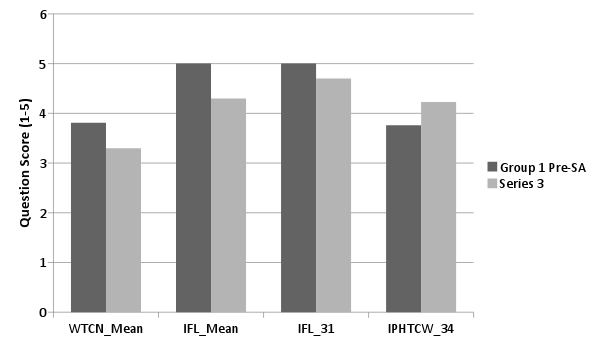
\includegraphics[width=\textwidth]{figures/geoghegan-img1.png}

  \begin{tikzpicture}
    \begin{axis}[
	xlabel={},  
	ylabel={Question score (1--5)}, 
	axis lines*=left, 
        width  = .95\textwidth,
	height = .3\textheight,
	enlarge x limits=.25,
 	bar width=6mm,
    	nodes near coords, 
	xtick=data,
	x tick label style={},  
	ymin=0,
	ybar,
	symbolic x coords={WTCN\_Mean,IFL\_Mean,IFL\_31,IPHTCW\_34},
	legend style={at={(.8,.1)},anchor=south}
	]
	\addplot+[ybar,lsRichGreen!80!black,fill=lsRichGreen] plot coordinates {
	    (WTCN\_Mean, 3.81) (IFL\_Mean,5) (IFL\_31, 5) (IPHTCW\_34,3.76) 
	}; 
	\addplot+[ybar,lsMidBlue!80!black,fill=lsMidBlue] plot coordinates {
	    (WTCN\_Mean, 3.3) (IFL\_Mean,4.3) (IFL\_31, 4.7) (IPHTCW\_34,4.23) 
	}; 
	\legend{Group 1 Pre-SA,Group 2 Post-SA}
    \end{axis} 
  \end{tikzpicture} 
% \todo[inline]{provide correct values}  
\caption{{Results of RQ1.}}
\label{fig:geoghegan:graph2}
\end{figure}

\newpage 
In addition to comparing them to the Group 1 pre-SA students, the Group 2 end of SA students were also assessed using the comparison pairs ‘In General’ (IG) and ‘While  {Abroad}’ (WA), wherein students reflected on how they felt about issues in general and specifically while abroad, as outlined in the methodology section. Results of Wilcoxon signed-rank tests showed that, out of the 14 comparison pairs divided between ‘IG’ and ‘WA’, 4 pairs were statistically different (\tabref{tab:geoghegan:4}). 

\begin{table}
\begin{tabularx}{\textwidth}{rQQrrrr}
\lsptoprule

\bfseries Pair & \bfseries In General & \bfseries While  {Abroad} & \bfseries \textit{T} & \bfseries z & \bfseries \textit{p} & \bfseries \textit{n$^2$}\\
\midrule
1 & 37. Using Eng/Fr/Ger in front of people in Spain makes me feel like I will be thought of as less \ili{Spanish}. & 15. Using Eng/Fr/Ger in front of people on Erasmus makes me feel like I will be thought of as less \ili{Spanish}. & 713.500 & 5.032 & .000 & 11.788\\
2 & 53. If I could speak Eng/Fr/Ger well, I could get to know more people from other countries. & 26. If I could speak Eng/Fr/Ger well, I could get to know more people from other countries while on my Erasmus. & 41.000 & 3.624 & .000 & 11.596\\
3 & 21. In the future, I would rather have a job in my home country than abroad. & 9. I would rather stay in my home country than live abroad. & 352.500 & 4.041 & .000 & 8.036\\
4 & 16. I think I often feel anxious and ill at ease when I have to speak to someone in Eng/Fr/Ger. & 25. I think I often feel anxious and ill at ease when I have to speak Eng/Fr/Ger with a \isi{native speaker}. & 313.000 & {3.044} & .002 & 8.297\\
\lspbottomrule
\end{tabularx}
\caption{Comparison Pairs.}
\label{tab:geoghegan:4}
\end{table}

Pair 1 indicated that students felt they would be thought of as less \ili{Spanish} when using their \isi{L2} in Spain as compared to during their Erasmus. This suggests that students may perceive themselves to be more self-conscious about speaking their TL in their home country, given that they will not be presenting themselves as having a uniquely \ili{Spanish} identity. On the other hand, in an international setting, students may perceive themselves as being free to exhibit their \isi{multilingual} identity without any threat of loss of face. Pair 2 suggested that, while reflecting on being abroad, students were less inclined to believe speaking their \isi{L2} well was needed to communicate with people from other countries, which seems counter intuitive. This could be explained by the fact that WA, students may be exposed to more situations in which they could use their TL, meaning that they did not need to seek out such situations to the extent they would at home. In other words, simply being abroad provided more opportunities to interact in the \isi{target language}. This may have resulted in the students being less concerned with needing a high L2 proficiency level in order to meet people from other countries: simply being abroad would lead to these opportunities. Pair 3 indicated that in the future, students saw themselves working abroad more than simply living abroad. This suggests that students may have been more instrumentally motivated in this regard, thinking practically about their opportunities for economic advancement in the future. Pair 4 suggested that students were overall more anxious speaking to a \isi{native speaker} while abroad, as opposed to any other speaker in the TL. This finding is consistent with what is suggested in the literature (e.g. \citealt{Woodrow2006}).

 
\subsection{RQ2: English vs. other languages}


The second \isi{research question} in this study aimed to investigate whether there was an effect of a three-month study abroad on the motivation and identity of higher education students sojourning in an \ili{English}-speaking country as compared with a French- or \ili{German}-speaking country. In order to investigate this, Mann-Whitney U tests were also carried out in order to compare students who had sojourned, or planned to sojourn, in an \ili{English}-speaking country with those in a \ili{German}- or French-speaking country. Only 1 of the 14 categories, namely the \isi{Ideal L2 Self}, and 4 individual questions, were found to be significantly different when comparing the two factors, which once again demands caution in interpreting the results. \tabref{tab:geoghegan:5} below shows the descriptive statistics with the means, the standard deviation and the test statistics for the category and questions which yielded significant results. Two categories were relevant, namely the \isi{Ideal L2 Self} (IL2S) and intended leaning effort (ILE). Again, it should be borne in mind that higher values correspond to ‘strongly agree’ and ‘agree’ while lower values imply less agreement.

\begin{sidewaystable}
\begin{tabularx}{\textwidth}{Qrrrrrrrrr}
\lsptoprule

\bfseries Question & \multicolumn{2}{c}{\bfseries M} & \multicolumn{2}{c}{\bfseries SD} & \bfseries \textit{U} & \bfseries \textit{z} & \bfseries \textit{p} & \bfseries \textit{n\textsuperscript{2}} & \bfseries \textit{d}\\
& \bfseries Eng & \bfseries Fr/Ger & \bfseries Eng & \bfseries Fr/Ger &  &  &  &  & \\
\midrule 
IL2S\_Mean & 4.57 & 3.58 & 1.05 & 1.60 & 216.000 & 2.597 & .009 & 0.057 & 0.49\\
\tablevspace
IL2S\_42: In my future career, I imagine myself being able to use \ili{English}/French/\ili{German}. & 4.92 & 4.69 & .269 & .480 & 260.000 & 2.248 & .025 & 0.025 & 0.321\\
\tablevspace
ILE\_24:It is extremely important for me to learn \ili{English}/French/\ili{German}. & 4.69 & 4.38 & .643 & .650 & 239.000 & 2.040 & .041 & 0.041 & 0.411\\
\tablevspace
ILE\_4: If \ili{English}/French/\ili{German} were not taught in my home university, I would try to go to classes somewhere else. & 4.71 & 4.23 & .457 & .927 & 238.500 & 1.977 & .048 & 0.041 & 0.413\\
\tablevspace
ILE\_54: If an \ili{English}/French/\ili{German} course was offered in the future, I would like to take it. & 4.04 & 4.69 & 1.120 & .480 & 453.000 & 2.044 & .041 & 0.055 & 0.481\\
\lspbottomrule
\end{tabularx}
%%[Warning: Draw object ignored]
%%[Warning: Draw object ignored]%%please move \begin{table} just above \begin{tabular . 
\caption{Results of RQ2.}
\label{tab:geoghegan:5}
\end{sidewaystable}

Most importantly, the results show that the \ili{English} group scored higher overall with regards to \isi{Ideal L2 Self} (IL2S\_Mean), suggesting that those students focusing on learning \ili{English} could better visualise themselves as the \isi{L2} user they wished to be than those in the Fr/Ger group. One reason for this could be the fact that the \ili{English} group may simply believe that the English language is more important for their future given its role as an international language. Within this category, it was found that those in the \ili{English} group could imagine themselves using \ili{English} in their future career (IL2S\_42) to a greater extent than the French /\ili{German} group. This element of \isi{instrumental motivation} is not surprising given the importance that is placed on speaking \ili{English} for economic advancement, as mentioned above and discussed by \citet{BlockCameron2002}. Results also showed that while the \ili{English} group was more likely to take classes elsewhere if it was not possible to learn their TL in their home university (ILE\_4), the French/\ili{German} group was more likely to take a language course if it was offered in the future (ILE\_54). Finally, it was found that the \ili{English} group was significantly more likely to think that it was extremely important for them to learn their \isi{target language} (ILE\_24), again highlighting the importance placed on learning \ili{English}. \figref{fig:geoghegan:graph3} displays the values above in order to offer a visual presentation of the results, where higher values correspond to more agreement with the proposed statements.

\begin{figure}  
% 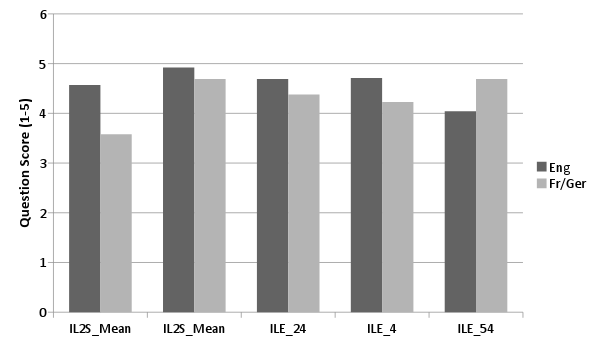
\includegraphics[width=\textwidth]{figures/geoghegan-img2.png}

  \begin{tikzpicture}
    \begin{axis}[
	xlabel={},  
	ylabel={Question score (1--5)}, 
	axis lines*=left, 
        width  = .95\textwidth,
	height = .3\textheight,
% 	enlarge x limits=.25,
 	bar width=6mm,
    	nodes near coords, 
	xtick=data,
	x tick label style={},  
	ymin=0,
	ybar,
	symbolic x coords={IL2S\_Mean,IL2S\_42\_Mean,ILE\_24,ILE\_4,ILE\_54},
	legend style={at={(.8,.3)},anchor=north}
	]
	\addplot+[ybar,lsRichGreen!80!black,fill=lsRichGreen] plot coordinates {
	    (IL2S\_Mean,4.57) (IL2S\_42\_Mean,4.92) (ILE\_24,4.69) (ILE\_4,4.71) (ILE\_54,4.04) 
	}; 
	\addplot+[ybar,lsMidBlue!80!black,fill=lsMidBlue] plot coordinates {
	    (IL2S\_Mean,3.58) (IL2S\_42\_Mean,4.69) (ILE\_24,4.38) (ILE\_4,4.23) (ILE\_54,4.69) 
	}; 
	\legend{Eng,Fr/Ger}
    \end{axis} 
  \end{tikzpicture} 
% \todo[inline]{provide correct values}   
\caption{{Results of RQ2.}}
\label{fig:geoghegan:graph3}
\end{figure}



\section{Discussion}

Regarding RQ1, the results of the questionnaire pointed to a difference between Group 1 and 2 in two of the fourteen categories, and a difference between the \ili{English} and French/\ili{German} subgroups of Group 2 in just one of the fourteen categories. Results showed that the pre-SA Group 1 was significantly more likely to want to learn the \isi{foreign language} of the country they will be visiting and that their overall mean for interest in foreign languages was greater than that of end of SA Group 2. Group 2, however, was significantly more likely to have thoughts they wish to share with others of different nationalities, suggesting a higher level of international \isi{posture} in this regard. Finally, it was found that the pre-SA students were significantly more willing to communicate in their native language than in their \isi{target language}, whereas the end-of SA group was equally as likely to communicate in both languages. These findings are in accordance with the idea that SA offers a potential boost to the learner’s willingness to communicate, as well as a consequential development of a sense of belonging within an international community (\citealt{Juan-GarauEtAl2014}). Notably, regarding the remaining categories, no statistical difference was found, which suggests that a period of \isi{SA} may have little or no effect on dimensions such as fear of assimilation, instrumentality, language anxiety, \isi{L2} self confidence, international vocation or activities, interest in international news and WTC in the TL. At this point, it should again be noted that in order to address this \isi{research question}, a cross-sectional approach was taken. It is important to take this into consideration when discussing the results, and highlight the benefit of carrying out a similar study with a longitudinal approach in order to determine whether similar findings would arise. As for RQ2, comparing Group 2 students sojourning in an \ili{English}-speaking country with those in a \ili{German}- or French-speaking country, it was found that the \ili{English} group considered learning their TL to be extremely important, and that students could imagine themselves using this language in their future careers to a significantly greater amount than the other groups. In other words, as suggested in the literature, there is a tendency for those learning a \isi{lingua franca} such as \ili{English} to be increasingly instrumentally motivated (\citealt{BlockCameron2002}). In addition, this group appeared to be better able to visualise themselves as the \isi{L2} users they wished to be than the French/\ili{German} group, having a statistically higher score in the \isi{Ideal L2 Self} mean. Finally, while the French/\ili{German} group was more likely to take a language course if it was offered in the future, the \ili{English} group was found to be more likely to take classes elsewhere (e.g. in a private language academy) if it was not possible to learn their TL in their home university. In these different ways, both groups appeared to show an interest in improving their formal language learning outside of the university setting. Again, despite these differences, a far greater number of categories showed no significant difference. This suggests that while students who study in an \ili{English} compared with a non-\ili{English} speaking country may differ in particular with regards to the \isi{Ideal L2 Self}, this appears not to be the case for the remaining dimensions. 
	The results of the questionnaire thus allow us to partially confirm our hypothesis, as only some categories resulted in a significant effect of a three-month SA on the language learning motivation and identity of higher education students, in particular regarding categories such as WTC in the native language and interest in foreign languages comparing pre-SA and end-SA (research question 1), and the Ideal L2 Self comparing the English group and the French/German group, (research question 2). 

The results suggest that those questions which did not reach a statistical difference may not have done so due to two main reasons (besides the obvious possibility that our sample was not large enough to achieve sufficient statistical power). Firstly, it is possible that the instrument itself was unable to capture the subtle changes in the individuals' motivation and identity during study abroad or across groups. As is suggested by \citet[318]{DeKeyser2014}, “much more detailed documentation is needed of how individual students are motivated for acquiring advanced language \isi{proficiency}” and “how this motivation increases or decreases during their stay abroad”. Secondly, it is possible that there simply was no difference between the two groups, given that students in each group generally achieved very high scores in each section. As the students were all enrolled in specialised language learning degrees it may be that the majority were just very highly motivated language learners, with no noticeable differences among the groups. This issue is also addressed in \citet[314]{DeKeyser2014} who points out that these language students who go on SA “are also quite motivated because language learning is what they are all about as translators/interpreters”. That is to say, there is a certain ceiling effect at hand, typical of learners at a more advanced stage \citep{Meara1994}. It should also be pointed out that participation was entirely voluntary, meaning that it is possible that only those students who were more motivated participated in the study. Thus, while the findings of the study reveal some interesting differences among the various groups, what is perhaps more noteworthy is this lack of differences found in the majority of the categories. Categories such as fear of assimilation, instrumentality, language anxiety, \isi{L2} self confidence, international vocation or activities, interest in international news and WTC in the TL showed no statistical difference both overall and in the individual questions. This is to say that neither the period of \isi{SA}, nor the country which they studied in, affected these issues. Future research would benefit from investigating whether similar results would be found in a longitudinal study, and from exploring the specific factors that affect, or do not affect, students regarding the categories addressed in this study. 


\section{Conclusions}

This study aimed to investigate the effect of SA on the motivation and identity of higher education students. The results show only a partial difference between the two groups who completed the questionnaire, perhaps, as suggested above, due to the overall high levels of motivation across the students, indicating that a more detailed investigation is required in order to discern significant differences between the groups, if they do exist.

Concerning the limitations of the study (besides the sample type), a further issue was the sample size of students focusing on learning French or \ili{German}. It was hoped that the groups would contain an equal number of students studying in each country. However, given the demand by students, the majority of placements were in \ili{English}-speaking countries.

While individually the fields of SA, identity, motivation and \isi{ELF}, as well as the theory of the \isi{L2} \isi{motivational} self system, have been studied extensively, relatively little has been done so far to investigate how these elements interact. This study has taken the initial steps towards understanding the effect of SA, on an array of factors pertaining to motivation and identity, investigating in particular elements from the \isi{L2} \isi{motivational} self system, while also aiming to gain a preliminary understanding of the effect of \isi{ELF} on these issues. It has been suggested that while a period of SA may have a positive impact on learners' \isi{WTC} in the NL and interest in FL, it may have no effect on the other issues that were investigated. Furthermore, when comparing those studying abroad in an \ili{English}/non-\ili{English}-speaking country, differences were found in particular with regards to the category of the \isi{Ideal L2 Self}, with participants showing similarities in the other categories.

\newpage 
As highlighted above, a more detailed investigation is needed alongside the quantitative analysis in order to fully understand and discern the similarities and differences between the groups. With this in mind, in order to gain a more thorough understanding of the development and negotiation of the learner’s ongoing motivational process during SA \citep{Kim2009}, in \citet{GeogheganPerezVidalForthcoming}, a follow-up study is carried out, adopting qualitative tools in order to provide this more detailed investigation. 
 
\section*{Appendix 1: Questionnaire content}
\sloppy 

We would like to ask you to help us by answering the following questions~concerning language learning in \isi{Study Abroad}, and people's feelings about languages and communication in general. This is not a test so there are no 'right' or 'wrong' answers. We are interested in your personal opinion. Please give your answers sincerely as only this will guarantee the success of the investigation. Thank you very much for your help!~

\subsection*{Section 1} 

\textbf{First, would you please answer a few personal details and general information – we need this information to be able to interpret your answers properly.} 

\begin{enumerate}
\item 
What is your name?



\item 
What is your age (in years)?
\item 
What degree are you studying?
\item 
What foreign languages are you studying as part of your degree? Please write the language, how old you were when you started learning, and your level. e.g. {English} (6, B2.2) = (I am learning {English}. I started learning {English} when I was 6 years old. My level is B2.2) French (11, B1.1) = (I am learning French. I started learning French when I was 11 years old. My level is B1.1)
\item 
In what country are you doing your Erasmus?
\item 
Why did you choose this country/language to do your Erasmus?
\item 
Before this Erasmus, had you ever spent a period of time in a foreign country? If yes, where and for how long (in weeks)? Please include all trips e.g. 1. England (2 weeks) summer 2010, 2. England (4 weeks) summer 2011, 3. Germany (1 week) summer family trip 2011, etc.

\end{enumerate}

\subsection*{Section 2}

\textbf{In this section, there are going to be questions concerning interpersonal communication in everyday and classroom situations, using your native language, or the language you are learning. In some questions, you will be given the option {English}/French/{German}.~Please answer ONLY with regards to the language of the country where you are abroad (i.e. French if you are in France, German if you are in Germany or English if you are in an {English}-speaking country).}

Q1. How likely would you be to initiate communication in your native language in the following situations?

\begin{enumerate}
\item Talking with an acquaintance while waiting for the bus. (2)
\item Talking with a salesperson in a store. (3)
\item Talking in a small group of strangers. (4)
\item Talking with a friend while waiting for the bus. (5)
\item Talking with a stranger while waiting for the bus. (6)
\item Talking in a small group of acquaintances. (7)
\item Volunteering to make a presentation in front of a large group. (8)
\item Being the first one to speak while doing group work. (9)
\item Asking the teacher a question in front of the class. (10)
\end{enumerate}


Q2. How likely would you be to initiate communication in {English}/French/{Ger\-man} in the following situations?

\begin{enumerate}
\item Talking with an acquaintance while waiting for the bus. (2)
\item Talking with a salesperson in a store. (3)
\item Talking in a small group of strangers. (4)
\item Talking with a friend while waiting for the bus. (5)
\item Talking with a stranger while waiting for the bus. (6)
\item Talking in a small group of acquaintances. (7)
\item Volunteering to make a presentation in front of a large group. (1)
\item Being the first one to speak while doing group work. (8)
\item Asking the teacher a question in front of the class. (9)
\end{enumerate}

Q3. This section is about the importance and usefulness of languages in the world.

\begin{enumerate}
\item How much do you think knowing {English}/French/{German} would help you to become a more knowledgeable person? (1)
\item How much do you think {English}/French/{German} would help you if you travelled abroad in the future? (2)
\item How much do you think {English}/French/{German} would help your future career? (3)
\item To what extent do you think {English}/French/{German} is important in the world these days? (4)
\end{enumerate}


\subsection*{Section 3.1} 

\textbf{Finally, in this last section, we would like to know to what extent the statements included describe your own feelings or~situation. After each statement you’ll find five options. Please select the option~which best expresses how true the statement is about your feelings or situation.~For example, if the first~statement~was "I like skiing" and you like skiing very much, select the first~option. Remember: In some questions, you will be given the option {English}/French/{German}.~Please answer ONLY with regards to the language of the country where you are abroad (i.e. French if you are in France, German if you are in Germany or English if you are in an {English}-speaking country). First, think about how you feel while you are studying abroad and answering this questionnaire.}


\begin{enumerate}
\item  While abroad, I take every opportunity I can to speak {English}/French/\linebreak{Ger\-man} with international friends. (66)
\item  I’m not very good at volunteering answers in my classes in {English}/French/\linebreak{Ger\-man}. (67)
\item  I often read newspapers and watch tv news in the language of the country I am staying. (68)
\item  I think that my writing ability has improved the most during this Erasmus. (88)
\item  When I first arrived, I found it more difficult to learn {English}/French/\linebreak{Ger\-man} while on Erasmus than while at home. (69)
\item  When I first arrived, I found it more difficult to learn {English}/French/\linebreak{Ger\-man} than halfway through my Erasmus. (93)
\item  I am worried that other speakers of {English}/French/{German} would find my {English}/French/{German} strange. (70)
\item  I try to avoid talking with native {English}/French/{German} speakers if I can. (71)
\item  I would rather stay in my home country than live abroad. (72)
\item  I would not like to live with someone of a different nationality than me. (73)
\item  Halfway through my Erasmus, I thought it was easier to learn {English}/\linebreak{}French/{German} abroad than at home. (74)
\item  I think I would be studying {English}/French/{German} even if it weren’t compulsory. (75)
\item  I worry that native speakers will laugh at me when I speak {English}/French/\linebreak{German}. (76)
\item I think that my reading ability has improved the most during this Erasmus. (92)
\item  Using {English}/French/{German} in front of people on Erasmus makes me feel like I will be thought of as less {Spanish}. (77)
\item  I think I often feel anxious and ill at ease when I have to speak to someone in {English}/French/{German}. (78)
\item  I would get tense if someone asked me for directions in {English}/French/{German}. (79)
\item  I think that my speaking ability has improved the most during this Erasmus. (89)
\item  Whenever I think of my future career, I imagine myself being able to use {English}/French/{Ger\-man}. (80)
\item  I think that my listening ability has improved the most during this Erasmus. (90)
\item  I’m interested in the news of the country where I’m staying. (81)
\item  In the future, I want to work in a foreign country. (82)
\item  I get nervous and confused when I am speaking in my {English}/French/\linebreak{German} classes. (83)
\item  I think that my \isi{pronunciation} has improved the most during this Erasmus. (91)
\item  I can honestly say that I am really doing my best to learn {English}/French/\linebreak{German} while on my Erasmus. (84)
\item  If I could speak {English}/French/{German} well, I could get to know more people from other countries while on my Erasmus. (85)
\item  {English}/French/{German} ability would help me get a better paying job. (86)
\item  Now that I'm at the end of my Erasmus, I think it is easier to learn {English}/French/{German} at home than abroad. (87)
\item  Now that I'm at the end of my Erasmus, I think that it is more difficult to learn {English}/French {German} than I did halfway through. (94)
\item  I am more eager to return home now than I was halfway through my Erasmus. (95)
\end{enumerate}

\subsection*{Section 3.2}

\textbf{Now,} \textbf{think} \textbf{about} \textbf{how} \textbf{you} \textbf{feel} \textbf{IN} \textbf{GENERAL} \textbf{about} \textbf{each} \textbf{of} \textbf{these} \textbf{statements.}

\begin{enumerate}
\item 1. I often read newspapers and watch TV news about foreign countries (123)
\item If I made the effort, I could learn a new \isi{foreign language}. (124)
\item I would feel somewhat uncomfortable if a foreigner moved in next door. (125)
\item If {English}/French/{German} were not taught in my home university, I would try to go to classes somewhere else. (126)
\item I can imagine speaking {English}/French/{German} with international friends in my home country. (127)
\item I’m not very good at volunteering answers in our {English}/French/\linebreak{Ger\-man} language class in my home university. (128)
\item When I hear a song in {English}/French/{German}, I listen carefully and try to understand all the words. (129)
\item Learning a \isi{foreign language} is a difficult task for me. (130)
\item I have ideas about international issues, such as environmental issues and north-south issues. (131)
\item  I would like to be able to use {English}/French/{German} to get involved with people from other countries. (132)
\item  In the future, I would like to make friends with international students studying in my home country. (133)
\item  As a part of international society {Spanish} people must preserve the {Spanish} language and culture. (134)
\item  I have issues to address with people from different parts of the world. (135)
\item  I am sure I will be able to learn {English}/French/{German} to a high level. (136)
\item  Learning {English}/French/{German} is necessary because it is an international language. (137)
\item  Studying {English}/French/{German} will help me get a good job. (138)
\item  I always feel that my classmates speak {English}/French/{German} better than I do. (139)
\item  I don't think what's happening overseas has much to do with my daily life. (140)
\item  As \isi{internationalization} advances there is a danger of losing the {Spanish} language and culture. (141)
\item  When I think about my future, it is important that I use {English}/French/\linebreak{Ger\-man}. (142)
\item  In the future, I would rather have a job in my home country than abroad. (143)
\item  I think that {English}/French/{German} will help me meet more people. (144)
\item  I would like to be able to use {English}/French/{German} to communicate with people from other countries. (145)
\item  It is extremely important for me to learn {English}/French/{German}. (146)
\item  I feel uneasy speaking {English}/French/{German} with a \isi{native speaker}. (147)
\item  I have a strong interest in international affairs. (148)
\item  The things I want to do in the future require me to speak {English}/French/\linebreak{Ger\-man}. (149)
\item  If my dreams come true, I will use {English}/French/{German} effectively in the future. (150)
\item  I wouldn't mind sharing an apartment or room with an international student. (151)
\item  As a result of \isi{internationalization}, there is a danger {Spanish} people may forget the importance of {Spanish} culture. (152)
\item  If I were visiting a foreign country I would like to be able to speak its language. (153)
\item  Studying {English}/French/{German} will give me more opportunities. (154)
\item  In the future, I would like to participate in a volunteer activity to help foreigners living in the surrounding community. (155)
\item  I have thoughts that I want to share with people from other parts of the world. (156)
\item  I think I would study a \isi{foreign language} even if it weren’t compulsory. (157)
\item  I worry that the other students will laugh at me when I speak {English}/French/{Ger\-man}. (158)
\item  Using {English}/French/{German} in front of people in Spain makes me feel like I will be thought of as less {Spanish}. (159)
\item  A knowledge of {English}/French/{German} would make me a better educated person. (160)
\item  I would like to learn a lot of foreign languages. (161)
\item  I would talk to an international student if there was one in my class in my home university. (162)
\item  When I meet a speaker of {English}/French/{German}, I feel nervous. (163)
\item  In my future career, I imagine myself being able to use {English}/French/{German}. (164)
\item  I often imagine myself as someone who is able to speak {English}/French/{German}. (165)
\item  I'm not much interested in overseas news. (166)
\item  If I could have access to TV stations in {English}/French/{German}, I would try to watch them often. (167)
\item  I am the kind of person who makes great efforts to learn {English}/French/{German}. (168)
\item  I'm interested in an international career in the future. (169)
\item  For me to become an educated person, I should learn {English}/French/{German}. (170)
\item  I have no clear opinions about international issues. (171)
\item  I want to work in an international organization such as the United Nations. (172)
\item  I often talk about situations and events in foreign countries with my family and/or friends. (173)
\item  I can honestly say that I am really doing my best to learn {English}/French/\linebreak{Ger\-man}. (174)
\item  If I could speak {English}/French/{German} well, I could get to know more people from other countries. (175) 
\item { If an {English}/French/{German} course was offered in the future, I would like to take it. (177)}
\item  I am working hard at learning {English}/French/{German}. (178)
\item  In the future, {English}/French/{German} ability would help me get a better paying job. (179)
\end{enumerate}

\section*{ Appendix 2: Cronbach alpha values}

{\small
\begin{tabularx}{\textwidth}{>{\raggedright}p{3.1cm} >{\raggedleft}p{1.2cm}>{\raggedleft}p{2.5cm}>{\raggedleft}p{1.2cm}Y}
\lsptoprule

\bfseries Category & \bfseries Number of items & \bfseries Cronbach Alpha\newline (original study) & \bfseries Number of items & \bfseries \mbox{Cronbach Alpha}\newline (this study)\\
\midrule 
Fear of assimilation & 4 & {0.67}  & 4 & 0.651\\
\tablevspace
{Ideal} \isi{L2} self & 6 & {0.85}  & 4 & 0.761\\
\tablevspace
Instrumentality & 6 & {0.87}  & 6 & 0.759\\
\tablevspace
Intended learning effort & 8 & {0.86}  & 8 & 0.760\\
\tablevspace
Interest in foreign languages & 4 & {0.70}  & 3 & 0.629\\
\tablevspace
International contact & 4 & {0.87}  & 4 & 0.609\\
\tablevspace
Language anxiety & 3 & {0.81}  & 3 &  0.670\\
\tablevspace
{L2} self confidence & 4 & {0.57}  & 3 & 0.625\\
\tablevspace
Willingness to {communicate} in native language & 9 & {0.87}  & 9 & {0.}881\\
\tablevspace
Willingness to {communicate} in target language & 9 & {0.87} & 9 & {0.}916\\
\tablevspace
International posture: &  &  &  & \\
\tablevspace
Intergroup approach-avoidance tendency & 4 & 0.80 & 4 & 0.625\\
\tablevspace
International vocation or activities & 4 & 0.79 & 4 & 0.624\\
\tablevspace
Interest in international news & 5 & 0.76 & 5 & 0.676\\
\tablevspace
Having things to {communicate} to the world & 4 & 0.78 & 3 & 0.614\\
\lspbottomrule
\end{tabularx}
}
 
\sloppy
\printbibliography[heading=subbibliography,notkeyword=this] 
\end{document}